
\section{Procrustes}

\begin{frame}[fragile]
  \frametitle{Problema de Procrustes}
  \begin{figure}
    \centering
    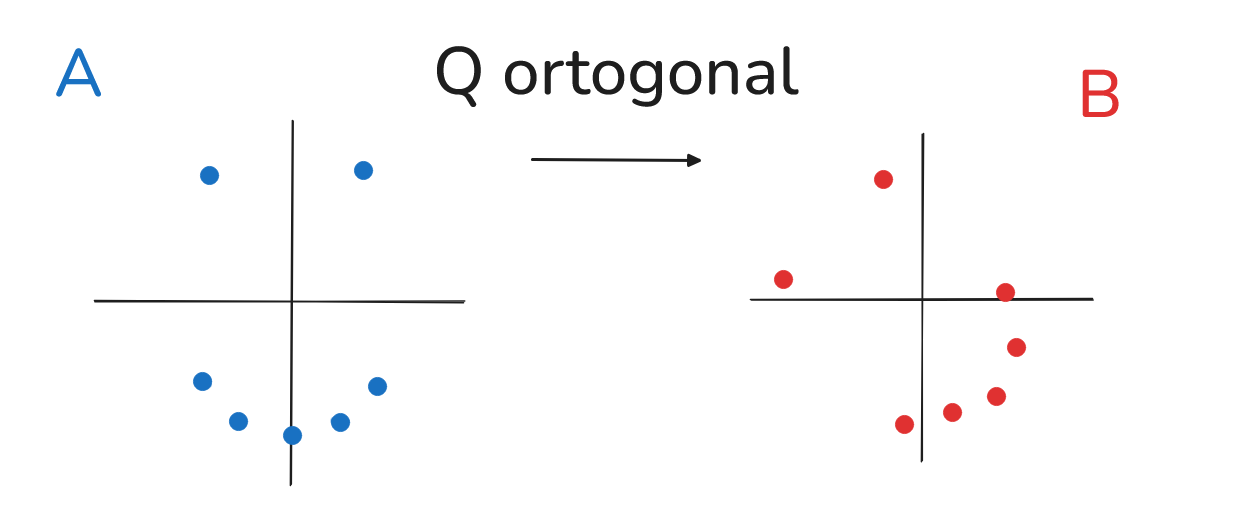
\includegraphics[width=0.75\textwidth]{procrustes.png}
  \end{figure}

  \[\argmin{Q} \fnorm{Q\blue{A} - \red{B}}^2 \text{  ou  } \argmin{Q} \sum_{i=1}^{n} \norm{Q\blue{a_i} - \red{b_i}}^2\]
\end{frame}

\begin{frame}[fragile]
  \frametitle{Problema de Procrustes com Translação}
  \begin{figure}
    \centering
    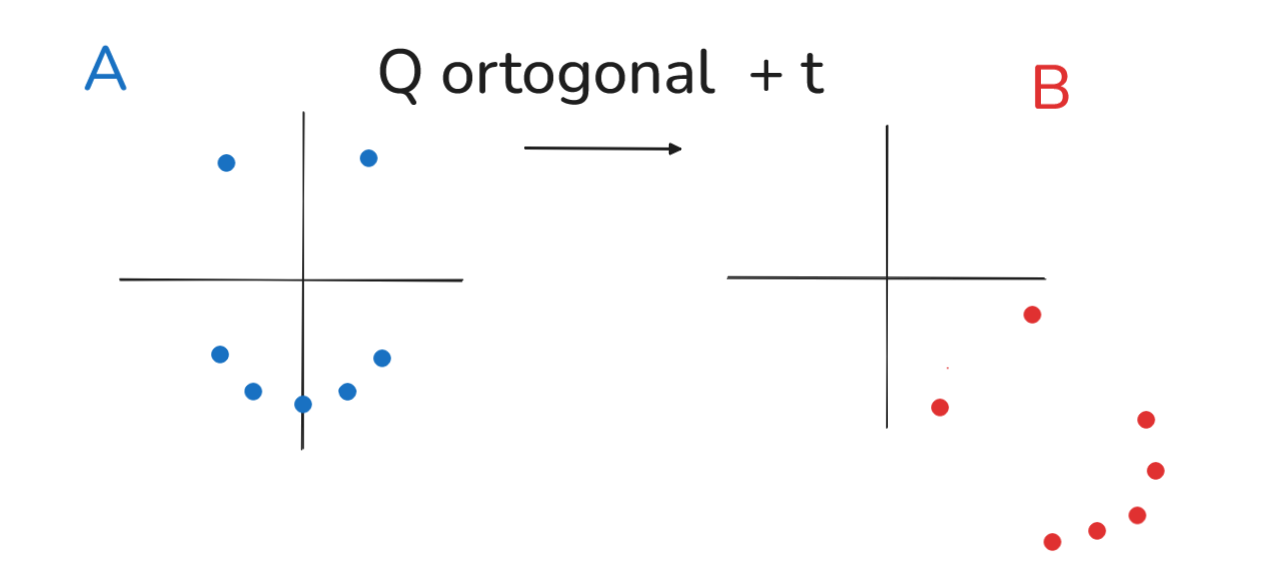
\includegraphics[width=0.75\textwidth]{procrustes-translated.png}
  \end{figure}

  \[\argmin{Q,t} \fnorm{Q\blue{A} + t e\t - \red{B}}^2\]

  \[e = \begin{bmatrix} 1 \\ \vdots \\ 1 \end{bmatrix}, \begin{bmatrix} \vert \\ t \\ \vert \end{bmatrix}\begin{bmatrix} 1 & \dots & 1 \end{bmatrix} = \begin{bmatrix} \vert & \vert & & \vert \\ t & t & \dots & t \\ \vert & \vert & & \vert \end{bmatrix}\]
\end{frame}

\begin{frame}
  \frametitle{Point Registration}
  \begin{figure}
    \centering
    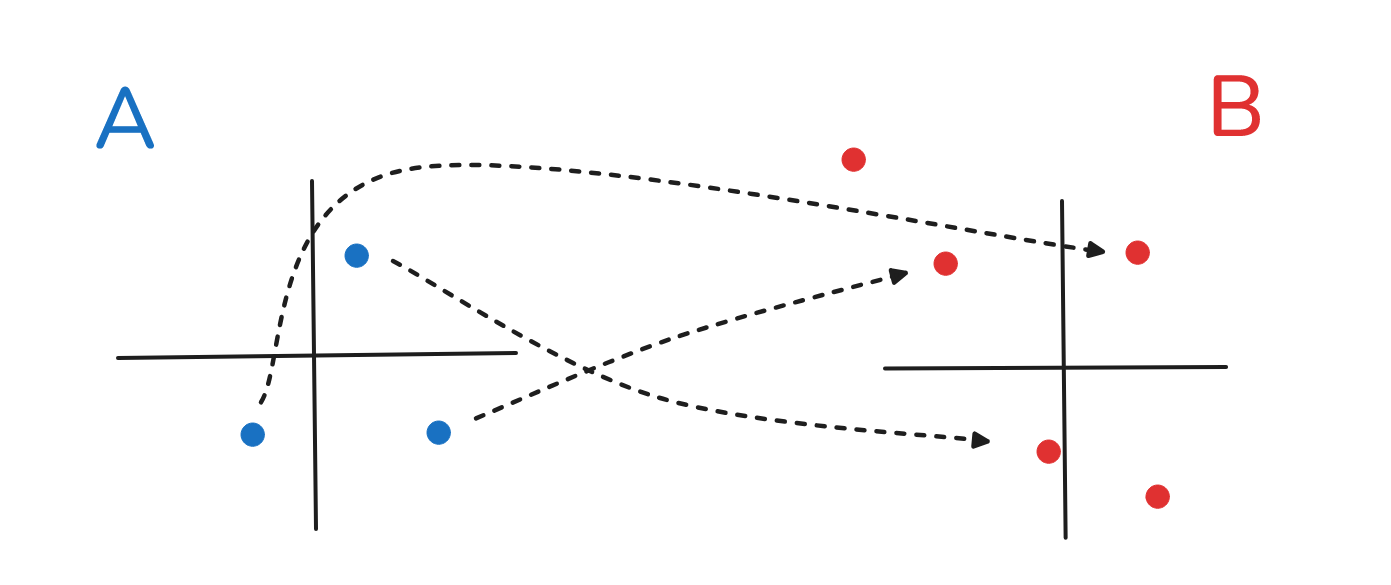
\includegraphics[width=1\textwidth]{point-registration.png}
  \end{figure}
\end{frame}

\begin{frame}
  \frametitle{Point Registration}
  \begin{center}
    Encontrar um mapeamento \[\blue{a_i} \to \red{b}_{\red{j}_{\blue{i}}}\]

    e $Q$ ortogonal minimizando

    \[\sum_{i=1}^{n} \norm{Q\blue{a_{i}} - \red{b}_{\red{j}_{\blue{i}}}}^2.\]
  \end{center}
\end{frame}
